%! TEX root = ../main.tex

Для проведения тестов, была написана простая демонстрационная программа.
Программа написана на языке C с использованием WinAPI. Ее интерфейс (рисунок
\ref{fig:interface}) представляет из себя два поля \verb!edit! для логина и для
серийного ключа. Серийный ключ генерируется из имени пользователя в процессе
работы программы.

\begin{figure}[h!]
  \centering
  \begin{subfigure}[bt]{0.45\textwidth}
    \centering
    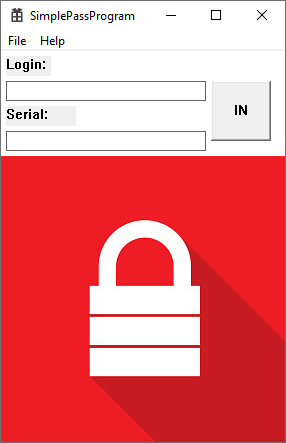
\includegraphics[width=\textwidth]{locked.png}
    \caption{}
  \end{subfigure}
  \hfill
  \begin{subfigure}[bt]{0.45\textwidth}
    \centering
    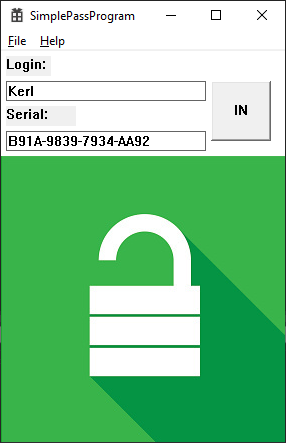
\includegraphics[width=\textwidth]{unlocked.png}
    \caption{}
  \end{subfigure}
  \caption{Интерфейс демонстрационной программы. а. --- заблокированное
    состояние; б. --- разблокированное состояние}
  \label{fig:interface}
\end{figure}

В случае, если введенный пользователем ключ не совпадает с тем, который
сгенерировала программа, выводится окно сообщения, уведомляющее пользователя о
неудаче. Данная уязвимость допущена здесь специально для большей
наглядности примера.

Для взлома данной программы воспользуемся отладчиком OllyDBG. Изменим исходный
код программы так, чтобы пользователь мог осуществить вход, введя любой пароль.

Для этого в памяти программы была найдена строка, которая выводится в окне
сообщения при неверном вводе ключа. А именно: "Invalid activation code".
Проследим по коду, предшествующему обращению к этой строке, условные переходы,
которые приводят к ситуации, когда программа остается заблокированной. Таким
образом легко обнаружить проверку двух строк на равенство. Очевидно в этом месте
происходит проверка ключа. На рисунке \ref{fig:disas_no_protect} видно, что по
адресу \verb!00FF143F! располагается проверка признака корректности ключа, после
чего идет условный переход на секцию кода, которая приводит к блокировке
приложения.

\begin{figure}[htpb]
  \centering
  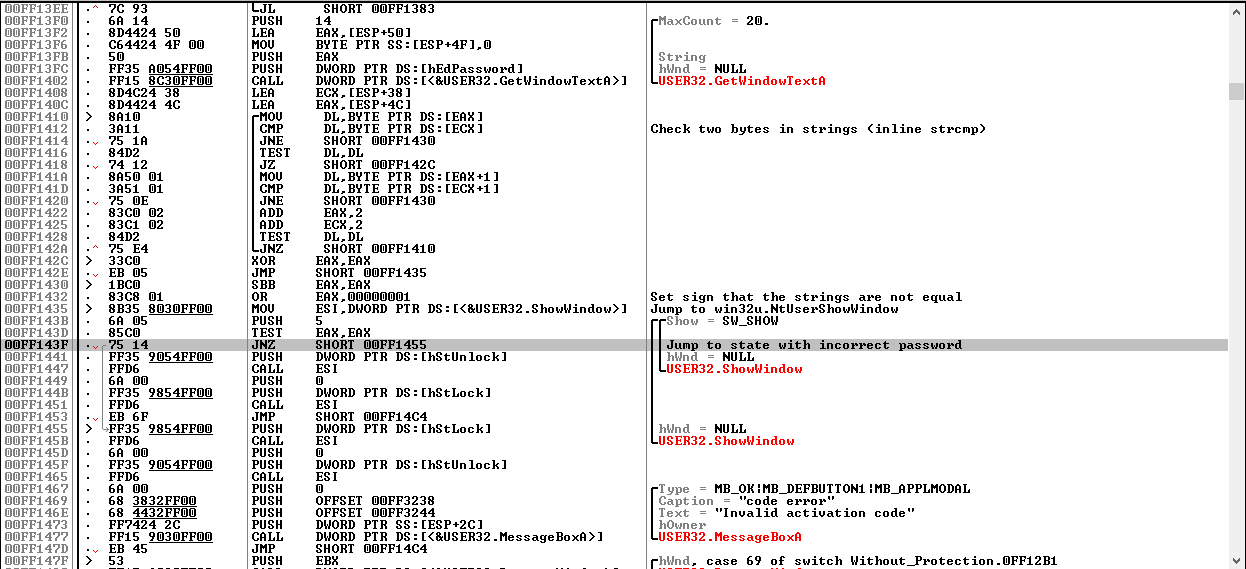
\includegraphics[width=\textwidth]{check_pass_section_croped.png}
  \caption{Окно отладчика при взломе программы без защиты}
  \label{fig:disas_no_protect}
\end{figure}

Так как наличие в регистре \verb!eax! значения отличного от нуля свидетельствует
о том, что введенный ключ не является корректным, оптимальным вариантом является
замена инструкции:
\begin{verbatim}
  test eax, eax
\end{verbatim}
на инструкцию
\begin{verbatim}
  xor eax, eax
\end{verbatim}
Таким образом в регистр \verb!eax! будет занесено значение 0, как и требует того
алгоритм программы при вводе корректного ключа. А условный переход выполняться
не будет .


На рисунке \ref{fig:cracked_unlock} представлена работа полученной таким образом
программы.
\begin{figure}[htpb]
  \centering
  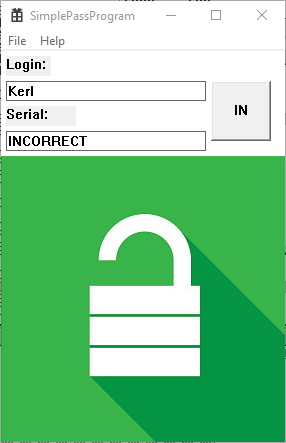
\includegraphics[width=0.4\textwidth]{cracked_unlocked.png}
  \caption{Работа взломанной программы}
  \label{fig:cracked_unlock}
\end{figure}

Теперь разместим в коде нашей программы разработанную ранее защиту от отладчика. 
Для этого создадим глобальную переменную:
\begin{verbatim}
  static const volatile DWORD CRC = 0x4C52454B;
\end{verbatim}
При помощи реализованных модулей вторая программа занесет в эту переменную
значение, равное контрольной сумме секции кода. Защиту разместим в участке кода,
который выполняется при нажатии на кнопку \verb!IN!. Если полученная контрольная
сумма не будет совпадать с эталонным значением, то будет выведено диалоговое
окно, сообщающее, что целостность кода была нарушена, а проверка пароля
выполняться не будет.

Стоит отметить, что уведомление пользователя об обнаружении отладчика или
нарушении целостности программы само по себе является уязвимостью. Такое
поведение реализовано исключительно в целях наглядности.

Исходный код программы претерпел незначительные изменения (рисунок
\ref{fig:protected_code}). Признак корректности ключа заносится в регистр
\verb!ecx! по адресу \verb!008B147B!.

\begin{figure}[htpb]
  \centering
  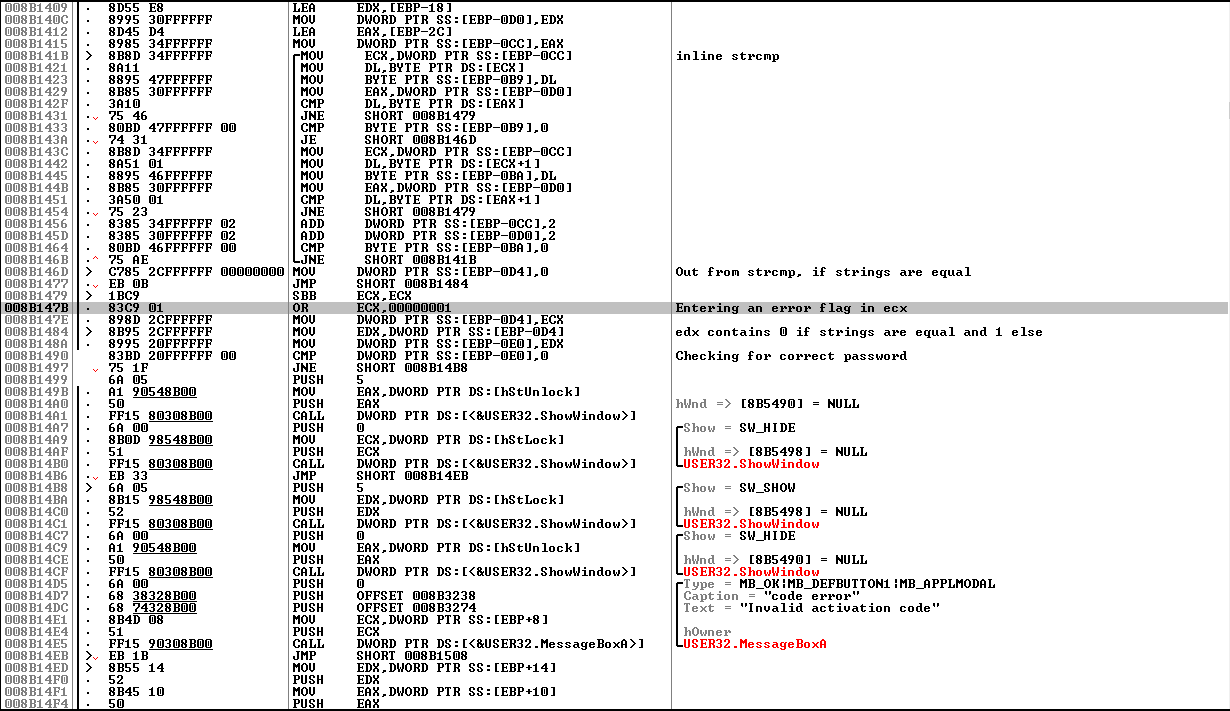
\includegraphics[width=\textwidth]{check_pass_section_protected_croped.png}
  \caption{Окно отладчика при взломе программы с защитой}
  \label{fig:protected_code}
\end{figure}

Для взлома программы заменим инструкцию
\begin{verbatim}
  or ecx, 1
\end{verbatim}
на инструкцию
\begin{verbatim}
  xor ecx, ecx  
\end{verbatim}

Так как полученная инструкция занимает на один байт меньше памяти,
освободившееся место заполним инструкцией \verb!nop!. Сохраним полученную
программу и попробуем ввести некорректное значение ключа.

\begin{figure}[hpbt]
  \centering
  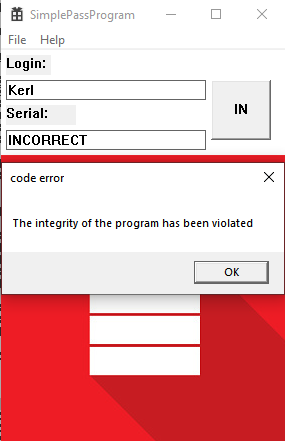
\includegraphics[width=0.4\textwidth]{Protection_work.png}
  \caption{Работа программы с защитой от взлома}
  \label{fig:protection_work}
\end{figure}

Как видно из рисунка \ref{fig:protection_work}, разработанная система
обеспечивает достойную защиту приложения.
%\newpage

Также стоит отметь, что если в отладчике установить точку останова, то он
занесет в первый байт инструкции значение \verb!CC!. Таким образом контрольная
сумма кода изменится и разработанный алгоритм позволяет это обнаружить. Данная
особенность защиты проиллюстрирована на рисунке \ref{fig:break_poin_catch}.

\begin{figure}[htpb]
  \centering
  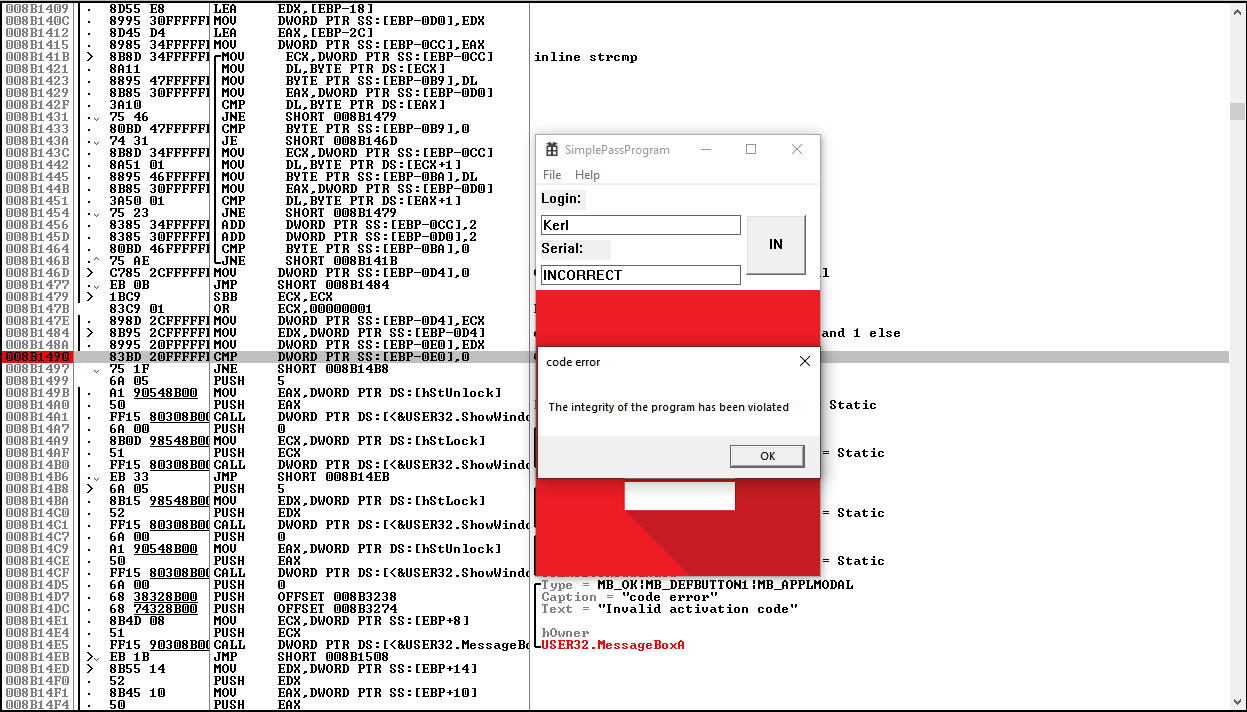
\includegraphics[width=0.8\textwidth]{Catch_breakpoint.png}
  \caption{Обнаружение системой защиты установленной точки останова}
  \label{fig:break_poin_catch}
\end{figure}

В ходе тестирования было выявлено, что при передачи различных регистров в
вызов макроса максимальная длина повторяющихся байт равна 9:
\begin{verbatim}
  0F 84 8B 00 00 00 EB EA FF
\end{verbatim}

Данные байты операции соответствуют двум инструкциям:
\begin{verbatim}
  je  no_section
  jmp section_loop
\end{verbatim}

Если повторяющаяся последовательность длинной в 9 байт покажется критичной,
можно вставить между этими инструкциями любую операцию с каким-либо регистром.
Например:
\begin{verbatim}
  xor ebx, ebx
\end{verbatim}

Результаты тестирования показывают, что реализованный метод обеспечивает защиту
программы от модификации исходного кода на должном уровне. Кроме того
реализованный метод препятствует процессу отладки. 
